\setlength{\columnsep}{3pt}
\begin{flushleft}

\begin{itemize}
	\item Cache is high speed storage area.
	\item Two types of cache are:
	\begin{itemize}
		\item \textbf{Memory cache} also called CPU memory:
		\begin{figure}[h!]
			\centering
			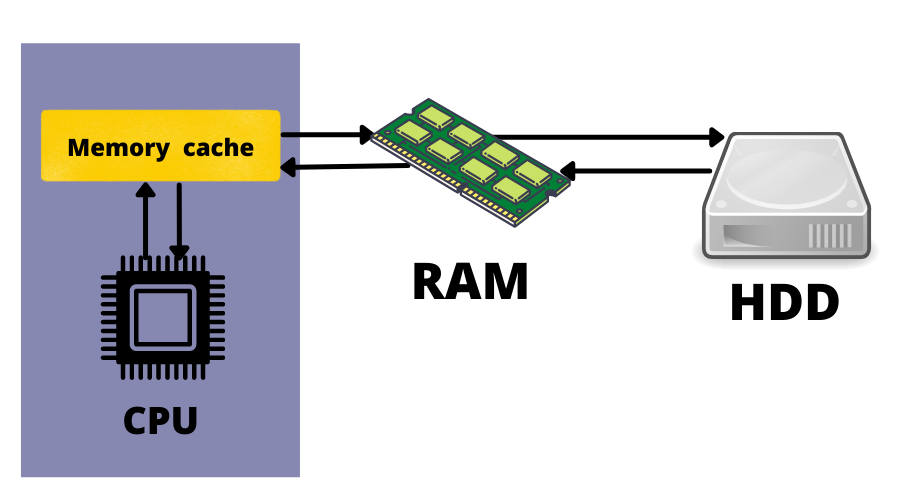
\includegraphics[scale=0.3]{content/chapter12/images/cache1.png}
			\caption{Memory cache}
			\label{fig:cache1}
		\end{figure}
		\begin{itemize}
			\item Memory cache is located inside the CPU.
			\item Multiple running processes stored their information in memory cache, instead of searching the disk everytime.
		\end{itemize}
		\item \textbf{Disk cache:} 
		\begin{figure}[h!]
			\centering
			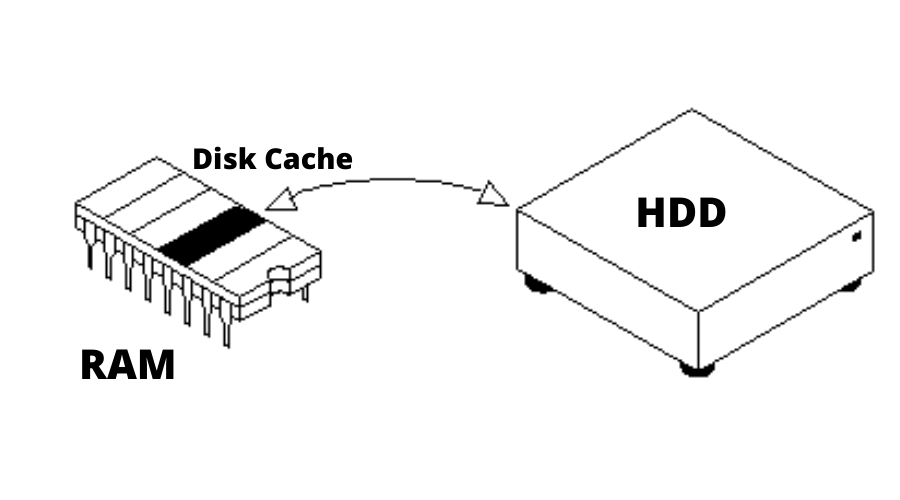
\includegraphics[scale=0.3]{content/chapter12/images/cache2.png}
			\caption{Disk cache}
			\label{fig:cache2}
		\end{figure}
		\begin{itemize}
			\item Disk cache can be part of the HDD or RAM. 
			\item Disk cache holds data that is frequently or recently read and is likely to be accessed next.
		\end{itemize}
	\end{itemize}
\end{itemize}

\end{flushleft}

\newpage


